\section{Discussie en Aanbevelingen}
De vorige bacheloreindprojectgroep beveelde een undo-functionaliteit aan \cite{bep2012nedtrain}. Ook wij zien zeker het voordeel van een undo-functionaliteit in, omdat bij het gebruik wel eens iets per ongeluk verwijderd of veranderd wordt. Aangezien de NedTrain Planner nu meer wordt gebruikt voor onderzoek en educatie wordt de focus gelegd op andere belangrijke features. Als deze tool gebruikt gaat worden door de planners van NedTrain is een undo-functionaliteit een musthave. 

We hebben onderzocht hoe deze feature gemaakt zou kunnen worden. Een voordeel is dat Qt een Undo Framework heeft, maar om dit te kunnen gebruiken moet er veel aan de code veranderd worden. Dan komen we meteen bij ons volgende aanbeveling.

De tweede aanbeveling is de code kwaliteit verbeteren. 

Als derde aanbeveling zou het goed zijn om de communicatie tussen de solver en de interface te verbeteren. De grootste snelheidswinst is nu te behalen in de communicatie tussen de NedTrain Planner en de solver. Er kan worden gekeken naar de uitvoer van de solver tijdelijk naar een bestand te schrijven en deze daarna in te lezen door de NedTrain Planner. Ook kan de hoeveel informatie dat wordt verstuurd van de solver naar de NedTrain Planner worden gereduceerd. De frames die worden getoond door de interface worden \'e\'en voor \'e\'en verstuurd vanaf de solver. Door steeds het verschil door te geven valt een relatief grote snelheidswinst te behalen.

Een vierde aanbeveling is een feature toe te voegen waarbij de resources zo eerlijk mogelijk verdeeld worden over de resource units. Dit is vooral handig voor personeel in de werkplaatsen van NedTrain. Zo kan elk personeelslid voor elk moment van de dag zien aan welk project hij of zij werkt en wanneer zijn of haar pauzes zijn. Dit kan visueel gemaakt kunnen worden door in plaats van het resource profile een schema zoals in Figuur \ref{fig:schema} te laten zien in de interface. Elke rij hoort bij een resource unit en elke kolom bij een tijdseenheid. Een groen ingekleurd vlak betekent dat de resource unit actief is.

\begin{figure}[H]
\centering
\ifx\du\undefined
  \newlength{\du}
\fi
\setlength{\du}{15\unitlength}
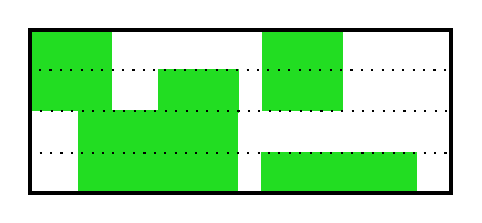
\begin{tikzpicture}
\pgftransformxscale{1.000000}
\pgftransformyscale{-1.000000}
\definecolor{dialinecolor}{rgb}{0.000000, 0.000000, 0.000000}
\pgfsetstrokecolor{dialinecolor}
\definecolor{dialinecolor}{rgb}{1.000000, 1.000000, 1.000000}
\pgfsetfillcolor{dialinecolor}
\pgfsetlinewidth{0.000000\du}
\pgfsetdash{}{0pt}
\pgfsetdash{}{0pt}
\pgfsetmiterjoin
\definecolor{dialinecolor}{rgb}{0.133333, 0.866667, 0.133333}
\pgfsetfillcolor{dialinecolor}
\fill (15.009342\du,3.062089\du)--(15.009342\du,5.007099\du)--(16.944819\du,5.007099\du)--(16.944819\du,3.062089\du)--cycle;
\definecolor{dialinecolor}{rgb}{0.133333, 0.866667, 0.133333}
\pgfsetstrokecolor{dialinecolor}
\draw (15.009342\du,3.062089\du)--(15.009342\du,5.007099\du)--(16.944819\du,5.007099\du)--(16.944819\du,3.062089\du)--cycle;
\pgfsetlinewidth{0.000000\du}
\pgfsetdash{}{0pt}
\pgfsetdash{}{0pt}
\pgfsetmiterjoin
\definecolor{dialinecolor}{rgb}{0.133333, 0.866667, 0.133333}
\pgfsetfillcolor{dialinecolor}
\fill (16.143460\du,5.003661\du)--(16.143460\du,6.976642\du)--(19.978780\du,6.976642\du)--(19.978780\du,5.003661\du)--cycle;
\definecolor{dialinecolor}{rgb}{0.133333, 0.866667, 0.133333}
\pgfsetstrokecolor{dialinecolor}
\draw (16.143460\du,5.003661\du)--(16.143460\du,6.976642\du)--(19.978780\du,6.976642\du)--(19.978780\du,5.003661\du)--cycle;
\pgfsetlinewidth{0.000000\du}
\pgfsetdash{}{0pt}
\pgfsetdash{}{0pt}
\pgfsetmiterjoin
\definecolor{dialinecolor}{rgb}{0.133333, 0.866667, 0.133333}
\pgfsetfillcolor{dialinecolor}
\fill (18.073891\du,4.011756\du)--(18.073891\du,5.036585\du)--(20.009369\du,5.036585\du)--(20.009369\du,4.011756\du)--cycle;
\definecolor{dialinecolor}{rgb}{0.133333, 0.866667, 0.133333}
\pgfsetstrokecolor{dialinecolor}
\draw (18.073891\du,4.011756\du)--(18.073891\du,5.036585\du)--(20.009369\du,5.036585\du)--(20.009369\du,4.011756\du)--cycle;
\pgfsetlinewidth{0.000000\du}
\pgfsetdash{}{0pt}
\pgfsetdash{}{0pt}
\pgfsetmiterjoin
\definecolor{dialinecolor}{rgb}{0.133333, 0.866667, 0.133333}
\pgfsetfillcolor{dialinecolor}
\fill (20.573271\du,3.027380\du)--(20.573271\du,5.007099\du)--(22.508749\du,5.007099\du)--(22.508749\du,3.027380\du)--cycle;
\definecolor{dialinecolor}{rgb}{0.133333, 0.866667, 0.133333}
\pgfsetstrokecolor{dialinecolor}
\draw (20.573271\du,3.027380\du)--(20.573271\du,5.007099\du)--(22.508749\du,5.007099\du)--(22.508749\du,3.027380\du)--cycle;
\pgfsetlinewidth{0.000000\du}
\pgfsetdash{}{0pt}
\pgfsetdash{}{0pt}
\pgfsetmiterjoin
\definecolor{dialinecolor}{rgb}{0.133333, 0.866667, 0.133333}
\pgfsetfillcolor{dialinecolor}
\fill (20.561233\du,6.012133\du)--(20.561233\du,6.976642\du)--(24.293391\du,6.976642\du)--(24.293391\du,6.012133\du)--cycle;
\definecolor{dialinecolor}{rgb}{0.133333, 0.866667, 0.133333}
\pgfsetstrokecolor{dialinecolor}
\draw (20.561233\du,6.012133\du)--(20.561233\du,6.976642\du)--(24.293391\du,6.976642\du)--(24.293391\du,6.012133\du)--cycle;
\pgfsetlinewidth{0.050000\du}
\pgfsetdash{{\pgflinewidth}{0.200000\du}}{0cm}
\pgfsetdash{{\pgflinewidth}{0.200000\du}}{0cm}
\pgfsetbuttcap
{
\definecolor{dialinecolor}{rgb}{0.000000, 0.000000, 0.000000}
\pgfsetfillcolor{dialinecolor}
% was here!!!
\definecolor{dialinecolor}{rgb}{0.000000, 0.000000, 0.000000}
\pgfsetstrokecolor{dialinecolor}
\draw (14.947591\du,4.010731\du)--(25.098698\du,4.010731\du);
}
\pgfsetlinewidth{0.050000\du}
\pgfsetdash{{\pgflinewidth}{0.200000\du}}{0cm}
\pgfsetdash{{\pgflinewidth}{0.200000\du}}{0cm}
\pgfsetbuttcap
{
\definecolor{dialinecolor}{rgb}{0.000000, 0.000000, 0.000000}
\pgfsetfillcolor{dialinecolor}
% was here!!!
\definecolor{dialinecolor}{rgb}{0.000000, 0.000000, 0.000000}
\pgfsetstrokecolor{dialinecolor}
\draw (14.962456\du,6.010054\du)--(25.113563\du,6.010054\du);
}
\pgfsetlinewidth{0.050000\du}
\pgfsetdash{{\pgflinewidth}{0.200000\du}}{0cm}
\pgfsetdash{{\pgflinewidth}{0.200000\du}}{0cm}
\pgfsetbuttcap
{
\definecolor{dialinecolor}{rgb}{0.000000, 0.000000, 0.000000}
\pgfsetfillcolor{dialinecolor}
% was here!!!
\definecolor{dialinecolor}{rgb}{0.000000, 0.000000, 0.000000}
\pgfsetstrokecolor{dialinecolor}
\draw (14.975737\du,5.015802\du)--(25.126844\du,5.015802\du);
}
\pgfsetlinewidth{0.100000\du}
\pgfsetdash{}{0pt}
\pgfsetdash{}{0pt}
\pgfsetmiterjoin
\definecolor{dialinecolor}{rgb}{0.000000, 0.000000, 0.000000}
\pgfsetstrokecolor{dialinecolor}
\draw (14.975737\du,3.050000\du)--(14.975737\du,6.981603\du)--(25.126844\du,6.981603\du)--(25.126844\du,3.050000\du)--cycle;
\end{tikzpicture}

\caption{Resource unit schema}
\label{fig:schema}
\end{figure}
